Here we present the system specifications such as which technologies we use in each component by drawing a new architecture diagram that specifies what technologies are used in each part of the system.

\section{Implementation first steps}
In this section we will describe out approach towards the implementation of the system, we will describe the process since the requirements
definition to the technological choices, some challenges and implementation details.

For gathering requirements we simply defined two groups, the first, the system Back-end has essential base functionalities, we focused only
on the essential without scoping or prioritizing, all the collected requirements are in the progress of being implemented, these include
web crawling modules, data mining for some data treatment and an extraction manager that allows remote calls of parameterized (granular) extractions.
In the system Front-end we followed a different approach by collecting a larger group of requirements that consist mainly in user interactions with the tool,
allowing us to narrow down the essential features based on requirements comparison. So at the end we sum up a few \textit{must have} requirements that
define the system identity an reflect the principles on which the project was designed upon (accessibility, simplicity, \glspl{osn} integration and contextual analysis).\\

\indent From here we built a simple \textit{proof of concept} that demonstrates the most basic of the workflow, this consists in a few steps that we next list:
\begin{itemize}
    \item \textbf{Back-end} - Extract users from a \glspl{osn} (for this particular case we used Facebook as source);
    \item \textbf{Service Aggregator} - Aggregate the extracted users in a graph respecting front end data contract;
    \item \textbf{Front-end} - Rendering a graph on the browser, allow simple interaction of node data display on the user mouse click.
\end{itemize}

\subsection*{Aside note}
As one may noticed in the previous list, for sake of objectivity we skipped the implementation of some pieces in the architecture,
namely, the network metrics \gls{api} and the data mining process, these will only be included in the full implementation, because for the current proof
of concept we labeled this components as complements (this may be seen as add ons or plugins that added to proof of concept will bring the
project to life).\\

\subsection{Proof of concept results}
\indent These steps previously listed steps prove that the designed architecture produces the expected results, furthermore we also conclude in an empiric way what are
the best tools and technologies that better suite the project requirements.\\

\begin{figure}[h!]
\begin{center}
  \hspace*{-0.8in}
  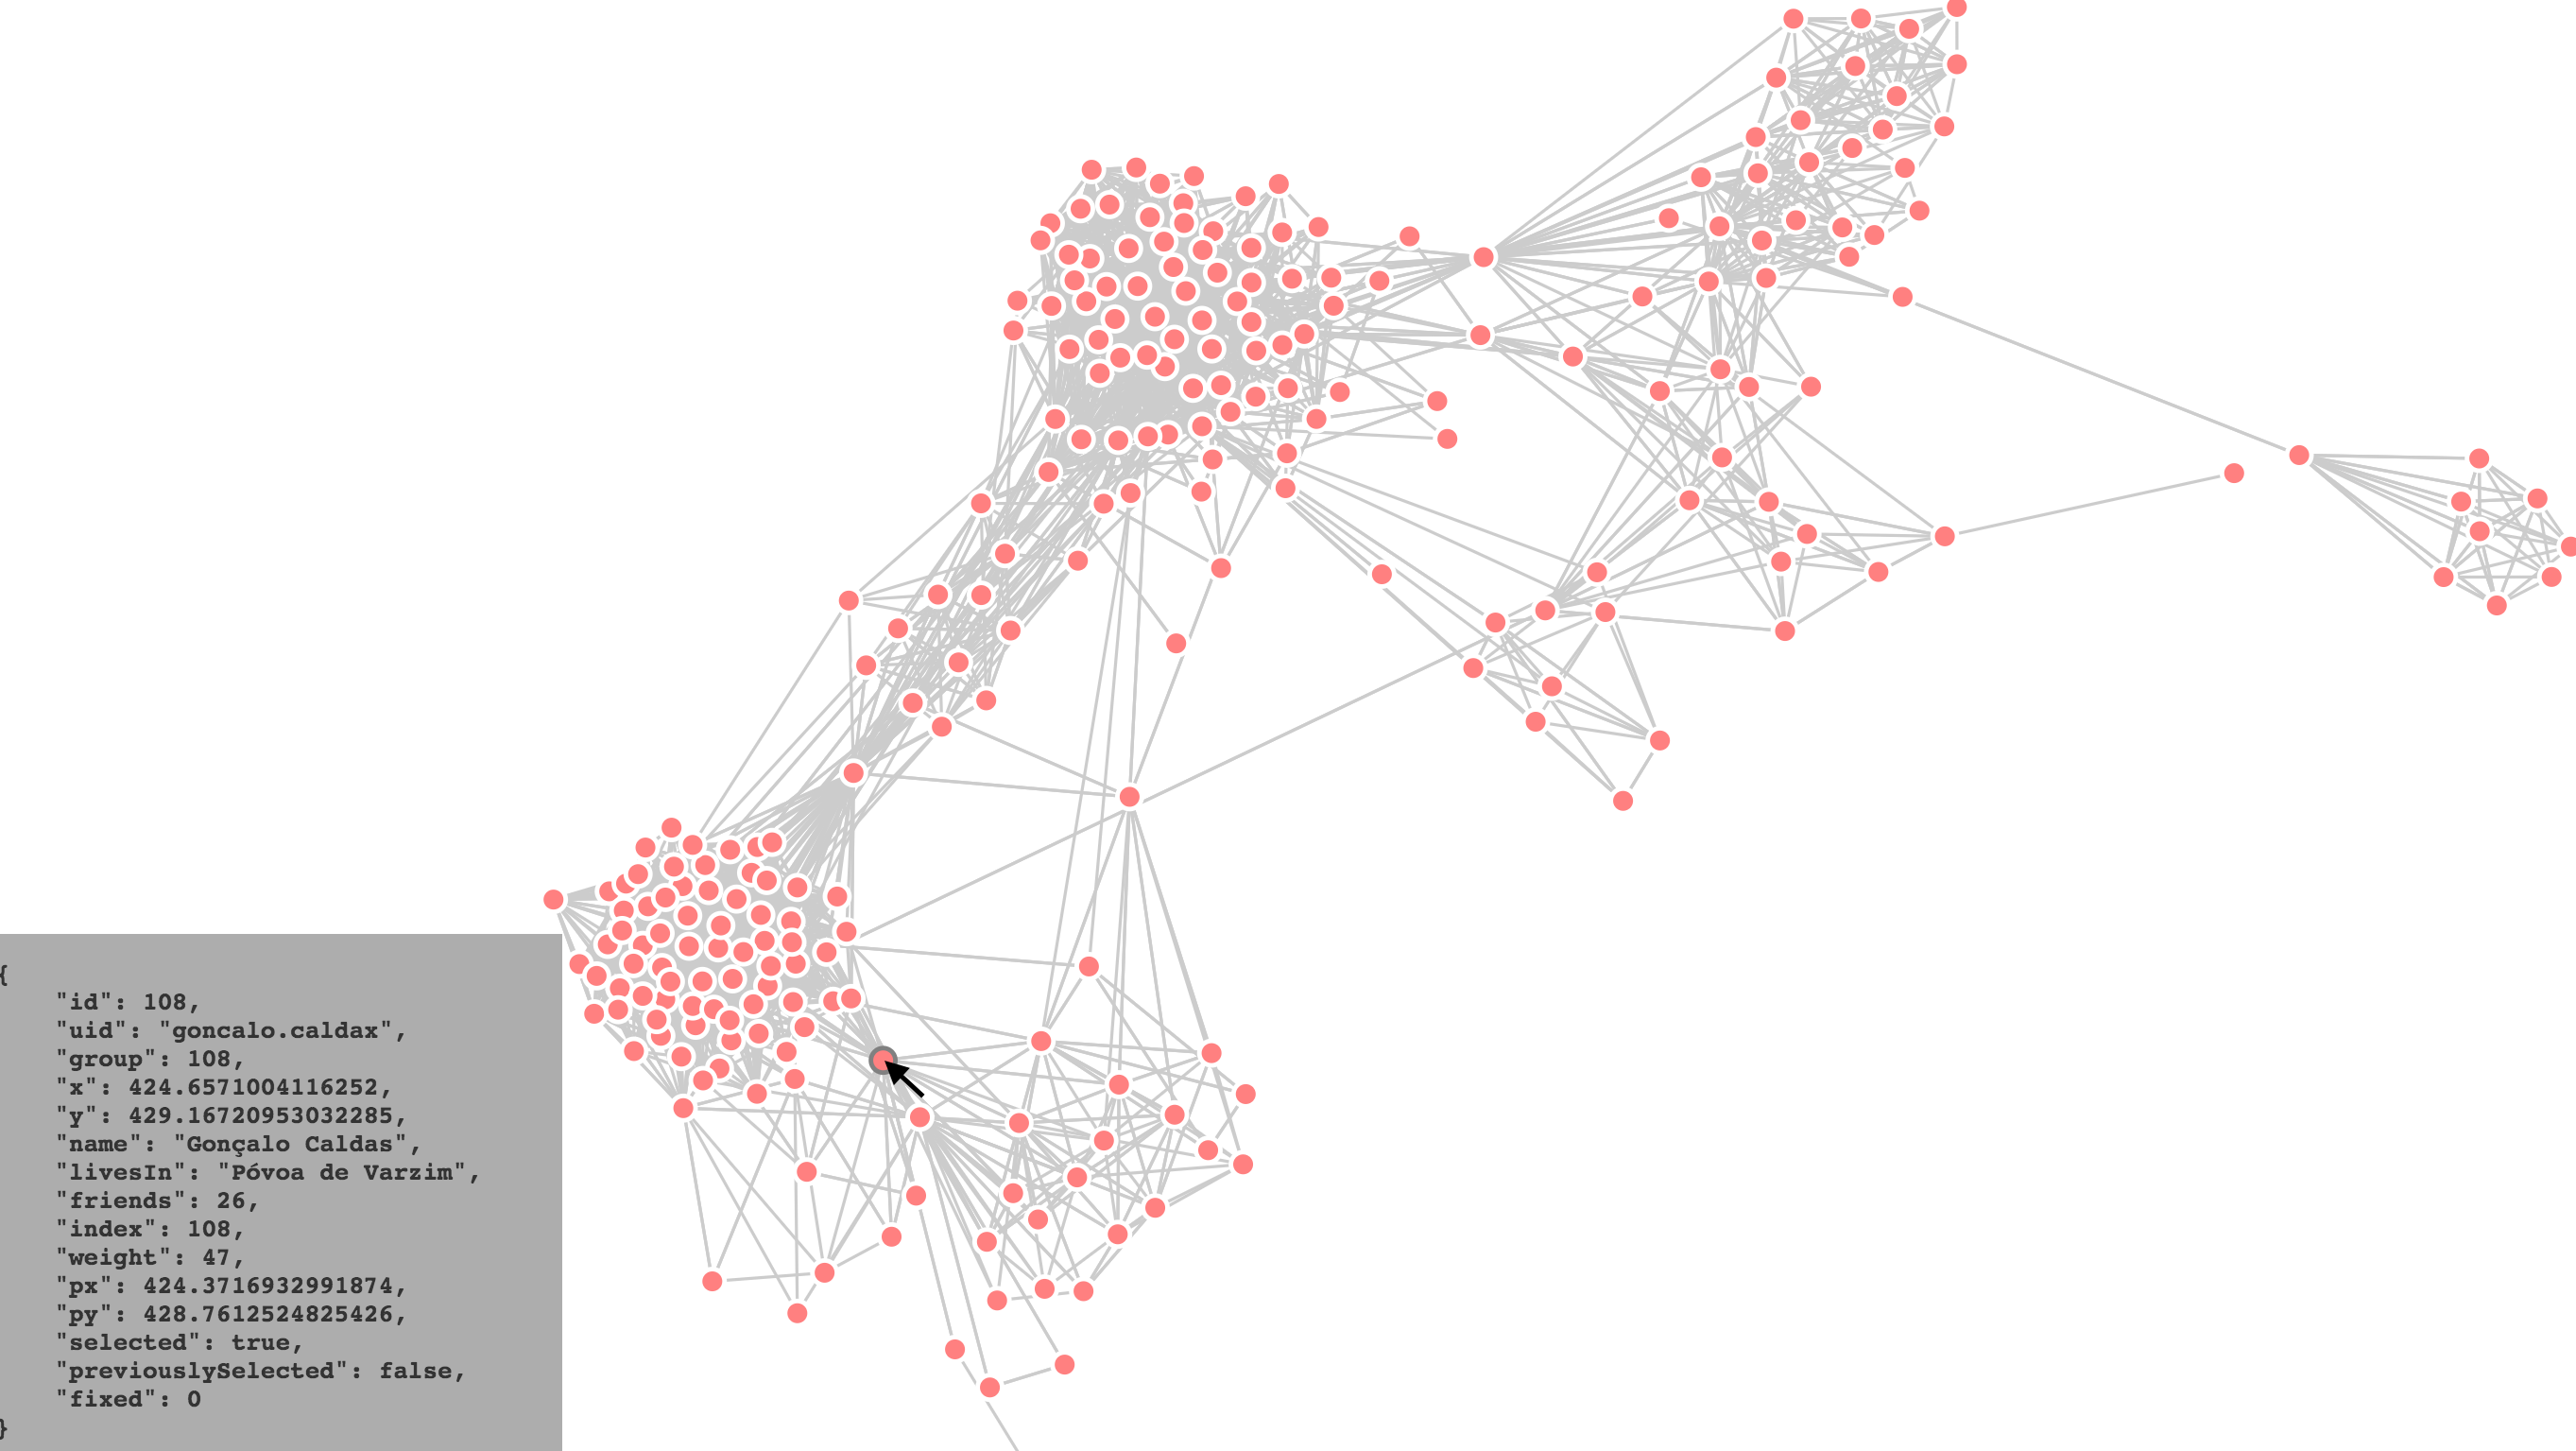
\includegraphics[width=1.2\textwidth]{img/proof-of-concept.png}
\end{center}
\caption{\label{img:poc} A \textit{screenshoot} of our first proof of concept.}
\end{figure}

\indent In the Figure \ref{img:poc}, we can observe a network being rendered, this represents the friendship network of a given user. Since there is an entry point user, if we let him in this network we would obtain a egocentric network that could not depict all the surrounding relations in this small society. What we did was remove this node in order to obtain more clarity to observe the network. At Figure \ref{img:poc} we also can see the interaction of clicking on a certain node and displaying the node information.

\section{Choose of Technologies}
Having the requirements been defined and a small proof of concept being developed as we see in the previous section, we are now able to present our technological choices and provide some context on how we came to these conclusions. We will divide the presentation into four main sections where we present technologies specific to an application layer, starting from database technologies until we reach the front end technologies. For each section we first list the technologies and then we present the motives that lead us to that specific choices.

\subsection{Database technologies}
\begin{itemize}
    \item \textbf{Neo4j};
    \item \textbf{MongoDB}.
\end{itemize}

Relational databases are one of the complex and advanced technologies that we have today. We have been building our applications on top of these technologies with very strict rules that allow our data to remain coherent trough applications lifetimes. Databases engines such as MySQL, PostgresSQL and SQL Server are good live examples of the relevance of these technologies. Meanwhile, applications have grown not just in size but also in complexity, the \textit{web era} came, and with it the need for tools that allow us to manage unstructured data. Other alternatives to relational databases have emerged, this are today known as \textbf{non relational databases} (also known as NoSQL databases). These are database engines that better allow us to store unstructured data or store data in a non relational way. The most suitable NoSQL database in the context of this project are graph databases such as \textbf{Neo4j} (\cite{developers2012neo4j}) that allows to think on data structures as graphs in the the more purest form. Also engines such as \textbf{MongoDB} (\cite{mongodb}) (a document oriented database, will give us more flexibility allowing us to have replicated data documents stored in a primary database and then migrate them into a graph database.

\subsection{Back-end technologies}
\begin{itemize}
    \item \textbf{Flask};
    \item \textbf{Python},
    \item \textbf{NetworkX};
    \item \textbf{PhantomJS};
    \item \textbf{Selenium WebDriver};
    \item \textbf{XPath}.
\end{itemize}

The main language that will supports our back-end is \textbf{Python}, this conclusion came very naturally since Python is one of the most used programming languages in the data science field along with others such as R or Java. We also choose Python for two other main reasons, first, we will be building data scrapper modules that need to simulate browser interactions, for that we will use \textbf{Selenium WebDriver} (\cite{documentation2013selenium}) for browser automation and interaction (with the complement of \textbf{PhantomJS}(\cite{hidayat2013phantomjs}) a headless browser with a Javascript API), and Python integrates very naturally with these technologies, along side with \textbf{XPath} (\cite{clark1999xml}) for querying HTML pages and narrow extraction to the essentials; second because \textbf{NetworkX} that (\cite{hagberg2013networkx}) was already presented in Chapter 4 it is written in Python and is a Python module. NetworkX is the most popular and powerful library that offers a large range of metrics and algorithms to run against graphs that come \textit{out of the box}.\\
\indent For networking, to make our back-end services available trough web \glspl{api}, we will use \textbf{flask} (\cite{ronacher2015flask}) a micro-framework for building simple networking applications in Python.

\subsection{Middleware technologies}
\begin{itemize}
    \item \textbf{NodeJS};
\end{itemize}

Sometimes we just need something very specific to perform nome networking middleware operations, for this purpose NodeJS (\cite{nodejs}) is an emerging technology
that has been famous for performing well this kind of tasks. For bridging between our back-end and front-end we might need some small pieces that act
as \textit{glue} between this two larger components, we will use NodeJS for that purpose.

\subsection{Front-end technologies}
\begin{itemize}
    \item \textbf{HTML};
    \item \textbf{Javascript}
    \item \textbf{CSS};
    \item \textbf{D3.js}.
\end{itemize}

Since we are building a web application, we automatically address to three main technologies that need no introduction, these are HTML, Javascript and CSS. In complement we will use for our specific needs that consists in building interactive graphs, a web data driven document representation system, \textbf{D3.js} (\cite{bostock2012d3}). In what concerns to visualization D3.js will be our main third party, that will bring us many features to help us on network representation and graph interaction \footnote{in our proof of concept we already used D3.js for rendering the network as we have demonstrated in Figure \ref{img:poc}}.
%
% \section{[PLACEHOLDER] Implementation architecture}
% ...
% \section{[PLACEHOLDER] Implementation details}
% ...
% \subsection{[PLACEHOLDER] Extraction and data mining}
% ...
% \subsection{[PLACEHOLDER] Network metrics}
% ...
% \subsection{[PLACEHOLDER] Front-end and service aggregator}
%
% \subsubsection{Graph render and interaction component}
% https://danielcaldas.github.io/react-d3-graph/sandbox/index.html
% Talk about the component, why it was built how it is going to be integrated in Socci tool.
